\documentclass{article}

\usepackage{fancyhdr}
\usepackage{extramarks}
\usepackage{amsmath}
\usepackage{amsthm}
\usepackage{amsfonts}
\usepackage{tikz}
\usepackage[plain]{algorithm}
\usepackage[noend]{algpseudocode}
\usepackage[ngerman]{babel}

\usepackage[utf8]{inputenc}
\usepackage{amsmath}
\usepackage{amsthm}
\usepackage{amsfonts}
\usepackage{amssymb}
\usepackage{graphicx}

\usepackage{listings}
\usepackage{color}

\definecolor{light-gray}{gray}{0.95}
\definecolor{keywords}{RGB}{255,0,90}
\definecolor{comments}{RGB}{20,20,113}
\definecolor{red}{RGB}{160,0,0}
\definecolor{green}{RGB}{20,150,50}


\lstset{ % General setup for the package
	language=Python,
	basicstyle=\small\ttfamily,
	numbers=left,
 	numberstyle=\small,
	frame=tb,
	tabsize=2,
	columns=fixed,
	showstringspaces=false,
	showtabs=false,
	commentstyle=\color{red},
	stringstyle=\color{green},
	keywordstyle=\color{blue},
	backgroundcolor=\color{light-gray},
	xleftmargin= 1.0cm,
	keepspaces=true,
	morekeywords={then, delete, downto, goto, change_state_to, ROW1}
}


\makeatletter
\def\BState{\State\hskip-\ALG@thistlm}
\makeatother


\usetikzlibrary{automata,positioning}

%
% Basic Document Settings
%

\topmargin=-0.45in
\evensidemargin=0in
\oddsidemargin=0in
\textwidth=6.5in
\textheight=9.0in
\headsep=0.25in

\linespread{1.1}

\pagestyle{fancy}
\lhead{\hmwkAuthorName}
\chead{\hmwkClass\ \hmwkClassInstructor\ \hmwkClassTime \hmwkTitle}
\rhead{\firstxmark}
\lfoot{\lastxmark}
\cfoot{\thepage}

\renewcommand\headrulewidth{0.4pt}
\renewcommand\footrulewidth{0.4pt}

\setlength\parindent{0pt}

%
% Create Problem Sections
%

\newcommand{\enterProblemHeader}[1]{
    \nobreak\extramarks{}{Aufgabenblatt \arabic{#1} continued on next page\ldots}\nobreak{}
    \nobreak\extramarks{Aufgabenblatt \arabic{#1} (continued)}{Aufgabenblatt \arabic{#1} continued on next page\ldots}\nobreak{}
}

\newcommand{\exitProblemHeader}[1]{
    \nobreak\extramarks{Aufgabenblatt \arabic{#1} (continued)}{Aufgabenblatt \arabic{#1} continued on next page\ldots}\nobreak{}
    \stepcounter{#1}
    \nobreak\extramarks{Aufgabenblatt \arabic{#1}}{}\nobreak{}
}

\setcounter{secnumdepth}{0}
\newcounter{partCounter}
\newcounter{homeworkProblemCounter}
\setcounter{homeworkProblemCounter}{4}
\nobreak\extramarks{Aufgabenblatt \arabic{homeworkProblemCounter}}{}\nobreak{}

%
% Homework Problem Environment
%
% This environment takes an optional argument. When given, it will adjust the
% problem counter. This is useful for when the problems given for your
% assignment aren't sequential. See the last 3 problems of this template for an
% example.
%
\newenvironment{homeworkProblem}[1][-1]{
    \ifnum#1>0
        \setcounter{homeworkProblemCounter}{#1}
    \fi
    \section{Aufgabenblatt \arabic{homeworkProblemCounter}}
    \setcounter{partCounter}{4}
    \enterProblemHeader{homeworkProblemCounter}
}{
    \exitProblemHeader{homeworkProblemCounter}
}

%
% Homework Details
%   - Title
%   - Due date
%   - Class
%   - Section/Time
%   - Instructor
%   - Author
%
%\newcommand{\hmwkTitle}{Aufgabe\ \#1}
\newcommand{\hmwkTitle}{Theoretische Informatik 1}
\newcommand{\hmwkDueDate}{}
\newcommand{\hmwkClass}{}
\newcommand{\hmwkClassTime}{}
\newcommand{\hmwkClassInstructor}{}
\newcommand{\hmwkAuthorName}{Dragan Runjaic 1030676, \\
				    Haris Ziko 1330011, \\
				    Peter Lorenz 1114658} 

%
% Title Page
%

\title{
    \vspace{2in}
    \textmd{\textbf{\hmwkClass:\ \hmwkTitle}}\\
    \normalsize\vspace{0.1in}\small{Due\ on\ \hmwkDueDate\ at 3:10pm}\\
    \vspace{0.1in}\large{\textit{\hmwkClassInstructor\ \hmwkClassTime}}
    \vspace{3in}
}

\author{\textbf{\hmwkAuthorName}}
\date{}

\renewcommand{\part}[1]{\textbf{\large Part \Alph{partCounter}}\stepcounter{partCounter}\\}

% Useful for algorithms
\newcommand{\alg}[1]{\textsc{\bfseries \footnotesize #1}}

% For derivatives
\newcommand{\deriv}[1]{\frac{\mathrm{d}}{\mathrm{d}x} (#1)}

% For partial derivatives
\newcommand{\pderiv}[2]{\frac{\partial}{\partial #1} (#2)}

% Integral dx
\newcommand{\dx}{\mathrm{d}x}

% Alias for the Solution section header
\newcommand{\solution}{\textbf{\large Solution}}

% Probability commands: Expectation, Variance, Covariance, Bias
\newcommand{\E}{\mathrm{E}}
\newcommand{\Var}{\mathrm{Var}}
\newcommand{\Cov}{\mathrm{Cov}}
\newcommand{\Bias}{\mathrm{Bias}}




\begin{document}
%\maketitle
%\pagebreak
 
 \newcommand{\TM}{\xrightarrow[\tau]{1}}
 \newcommand{\TMM}{\xrightarrow[\tau]{*}}
 
.  \newline

% Blatt 4 -----------------------------------------
\begin{homeworkProblem}
  \subsection{Pseudocode der NTM}
   %Die NTM geht zuerst läuft über das ganze Band und erzeugt weitere NTM bei jeder Raute. Wenn Sie an das Ende angelangt ist, verwirft sie. 
   %Die erzeugten TM bewegen sich zeitgleich an der Raute, wo sie erstellt wurden zum Anfang des jeweiligen $A(v_i)$ zurück. 
   
   %$$ A(v_1) \# A(v_2) \# \dots \#A(v_n) \#\#bin(k) $$ 
   
  % Nun kopiert jede NTM, das jeweilige $A(v_i)$ auf das zweite Band und schließlich wird $bin(k)$ auf das dritte Band der jeweiligen NTM 3 Mal kopiert.
  % Band 3 sieht dann so aus: $ \# bin(k) \# bin(k) \# bin(k) \# $, wobei das erste $bin(k)$ zum Aktualisieren des zweiten $bin(k)$, welcher 
  % die Anzahl der Elemente in $A(v_i)$, also $|bin(q_1)| \dots |bin(q_m)|$ überprüft, ob diese $\geq bin(k)$ sind. 
  % Der dritte  $bin(k)$ wird dekrementiert, wenn ein Knoten für eine Clique gefunden wurde. \\
   
	Um das CLIQUE Problem zu entscheiden benutzen wir eine Turingmaschine mit 2 Bändern. Im ersten Schritt werden alle Möglichkeiten betrachtet mit $n$ Knoten jeweils einen davon mit allen anderen zu verbinden. Dazu erstellen wir Turingmaschinen mit den Inputs $A(v_i)$ , $A(v_i)\#A(v_j)$, $A(v_i)\#A(v_j)\#A(v_l)$, \dots, wobei die Indizes von $v$ hier jeweils paarweise verschieden sein sollen. Das bedeutet $\sum_{k=1}^n \binom{n}{k} = 2^n$ viele Turingmaschinen wobei $k$ die Anzahl der aneinander gereihten Listen sein soll. Diese Möglichkeiten werden auf das zweite Band geschrieben und am ersten Band bleibt der Originalinput stehen. ( Die leere Turingmaschine wird sofort verworfen ) \\
	
   Danach wird die Binärzahl, die ganz rechts im Eingabeband steht, dupliziert und auf das Band 2 geschrieben ganz nach rechts geschrieben.
   Im nächsten Schritt wird die Anzahl der Knotenlisten, welche sich auf dem Band 2 befinden, abgezählt indem wir die kopierte zahl $k$ vom Band 1 als Hilfe benutzen.
   Wenn die Anzahl ungleich $k$ ist, dann wird die TM verworfen, weil eine Clique mit der Größe $k$ nur dann existieren kann, wenn in einer Menge von Knoten jeder mit jedem verbunden ist. ( daher wenn sie vollständig ist )  
   Dadurch stellen wir fest, dass es hierbei vermutlich um eine Clique handeln könnte. \\

   Der letzte Schritt ist es um zu überprüfen, ob in jeder Knotenliste, welche sich auf dem Band 2 befindet, $k$ Knoten vorkommen. 
   Dazu nehme man einen Knoten $v$ von der ersten Knotenliste und überprüfe, ob dieser Knoten $v$ in allen anderen Knotenlisten enthalten ist.\\

   \textbf{Notation.}  $|A(v_1)\# \dots A(v_i)\# \#A(v_n)\#| = l_g$, $|\#bin(k)| = l_k$, Inputlänge: $l_g + l_k = l$, $n$ \dots Anzahl der Knoten im Graph.
    
    \lstinputlisting[caption=Pseudocode zur NTM]{blatt4.py}
  
    \vfill
   % \begin{verbatim}
    %  Literatur: 
     
   % \end{verbatim}
    
    
    \subsection{Platzkomplexität}
    Um die Platzkomplexität zu bestimmen, betrachten wir zuerst die Codierung von den einzelnen Knoten an.
    Wir nehmen an, dass wir im Graph $n$ Knoten haben. Jeder Knoten ist in Binärdarstellung kodiert, d.h. jeder Knoten hat eine Länge 
    von $l = \lceil log_2 n \rceil$ mit der optimalen Kodierung. Nehmen wir an, dass wir einen Vollständigen Graphen $K_n$ hätte, welcher 
    wiederum eine Max-Clique darstellt.
    Laut der Kodierung von dem Graph braucht man n Zahlen für jede Knotenliste und Damit jeder Knoten mit jedem verbunden ist, braucht man 
    dazu noch $n$ Knotenlisten.
    
    Die Kodierung für einen Vollständigen Graphen würde folgendermaßen ausschauen:
    $$bin(v_1)-bin(q_{(1,1)})-bin(q_{(1,2)})-\dots-bin(q_{(1,n-1)})\#\dots\#bin(v_n)-bin(q_{(n,1)})-bin(q_{(n,2)})-\dots-bin(q_{(n,n-1)})\#\#bin(k)$$

    Der maximale Speicher wäre dann:
    $$S_T(n) = n * (n + n * l) = n * (n + n * \lceil log_2 n \rceil) = n^2 + n^2 * \lceil log_2 n \rceil = \mathcal{O}(n^2 * log n)$$
    

    Wir haben gezeigt, dass $S_{CLIQUE}(n) \in NSPACE$.
    

    \subsection{Zeitkomplexität}
     Für die Zeit werden wir uns wieder Beispiel mit dem vollständigen Graph betrachten, welches in der Platzkomplexität behandelt worden ist ( Da dies ja der worst case ist ).

    \paragraph{START GUESS and CHECK}
    Als erstes erzeugen wir $2^n$ Turingmaschinen um eine NTM zu simulieren. Für die Zeitanalyse entscheidend ist allerdings nur die Schleife, die über den gesamten Input iteriert. Dieser hat, wie bereits in der Speicherbedarfanalyse erläutert $n^2 \cdots \log(n)$ Länge. Damit folgt

 $$t_1(n) = \mathcal{O}(n^2 \cdot \log n)$$.

    \paragraph{CHECK LENGTH}
    Im nächsten Schritt wird nur eine Binärzahl dupliziert.
    
    $$t_2(n) = \mathcal{O}(\log n)$$

    \paragraph{DELETE RIGHT}
    Danach wird der rechte Teil auf dem Band 1 gelöscht.
    
     $$t_3(n) = \mathcal{O}(\log n)$$

    \paragraph{COPY LEFT VERTEX}
    Der letzte Schritt ist zu überprüfen, ob eine clique existiert. Für diese Berechnung ist das Kopieren eines Knoten notwendig. Dies ist in
    $$t_4(n) = \mathcal{O}(\log n)$$
    möglich. \\
    
    Als letztes werden  über beide Bänder für jeden zu überprüfenden Knoten (also maximal $n$ viele) von links nach rechts und nochmal von rechts nach links iteriert, damit man überprüft ob der Knoten $v$ in jeder Knotenliste enthalten ist.
     $$t_5(n) = \mathcal{O}(n \cdot n^2 \cdot log n) = \mathcal{O}(n^3 \cdot \log n)$$

    Die gesamte Zeitkomplexität ist dann gegeben durch:
    $$T(n) = t_1(n) + t_2(n) + t_3(n) + t_4(n) + t_5(n) = \mathcal{O}(n^2 \cdot \log n) + \mathcal{O}(\log n) + \mathcal{O}(\log n) + \mathcal{O}(\log n) + \mathcal{O}(n^3 \cdot \log n) = \mathcal{O}(n^3 \cdot \log n)$$

    Wir haben also gezeigt, dass $CLIQUE \in NP$ ist, da wir eine NTM haben, die $CLIQUE$ in polynomieller Zeit entscheiden kann.
     
\end{homeworkProblem}

\pagebreak

% Blatt 5 -----------------------------------------
\begin{homeworkProblem}
    \subsection{Zeigen Sie, dass P abgeschlossen gegenüber der Kleenschen Hülle ist.}


        Sei $A \in P$ eine Sprache. Wir zeigen nun, dass $A^* \in P$. Da $A\in P$ wissen wir, dass eine deterministische Turingmaschine $M_A$ existiert, die $A$ in polynomieller Zeit entscheidet. Wir werden nun mit Hilfe von $M_A$, $A^*$ in polynomieller Zeit wie folgt entscheiden:
    
    Zunächst bemerken wir, dass $w \in A^*$ dann und nur dann wenn, genau eine der Folgenden Eigenschaften gilt,
    
    \begin{enumerate}
    \item $w = \epsilon$
    \item $w \in A$
    \item $\exists u,v : w = uv \quad v,u \in A^*$,
    \end{enumerate}
     
     also entweder $w$ ist das 'leere' Wort oder ein Wort aus $A$ selbst oder zerlegbar in zwei Worte aus $A^*$.

Sei nun $w = a_1\dots a_n, a_i \in \Sigma$ und bezeichne $w_{ij}$ den Substring, der mit $a_i$ beginnt und mit $a_j$ endet. Wir erzeugen im folgenden Algorithmus eine Tabelle, sodass 

\begin{equation}
table(i,j)=\left\{
\begin{array}{cl} 
1, &  w_{i,j} \in A^*\\ 
0, & \mbox{sonst} .
\end{array}\right.
\end{equation}  

\begin{algorithm}
\caption{Entscheider}\label{euclid}
\begin{algorithmic}[1]
\If{$w=\epsilon$} \underline{accept} 
\Else
\For{$l\gets 1,n$}
\For{$i\gets 1,n-(l-1)$}
\State $j\gets i+l-1$
\State Run $M_A$ on $w_{i,j}$
\If{$M_A$ accepts $w_{i,j}$} 
$table(i,j) := 1$ 
\Else
\For{$k\gets i, j-1$}
\If{$table(i,k)= 1$ and $table(k+1,j) = 1$} 
$table(i,j) = 1$
\EndIf
\EndFor
\EndIf
\EndFor
\EndFor
\EndIf
\If{$table(1,n)= 1$} \underline{accept} \Else \, \underline{reject}
\EndIf
\end{algorithmic}
\end{algorithm}

Wir betrachten also alle möglichen Substrings von $w$, beginnend mit Substrings der Länge $1,2, \dots$ bis zum Substring der Länge $n$, also $w$ selbst. Zunächst testet der Algorithmus in Zeile 5, ob der Substring selbst entscheidbar ist, falls nicht, so nutzen wir die oben erwähnte Eigenschaft 3 in Zeile 8-10 um zu sehen ob das Wort in zwei von $M_A$ entscheidbare Worte zerlegbar ist. Letztendlich bleibt nur noch zu überprüfen, ob $table(1,n) = 1$ um zu entscheiden ob $w \in A^*$.

Wir haben also einen Algorithmus, der mit Hilfe von $M_A$ entscheiden kann ob $w \in A^*$ oder nicht. Bleibt nur noch zu Überprüfen ob er dies auch in polynomieller Zeit tut. Offensichtlich sind die drei For-Schleifen entscheidend für die Laufzeit im Algorithmus. Die dritte For-Schleife ruft $M_A$ und berücksichtigt man, dass $M_A$ in polynomieller Zeit entscheidet, also in $\mathbb{O}(n^k),k \geq 0$ so ergibt sich insgesamt eine Laufzeit von

\begin{eqnarray}
T(n) &=& \mathbb{O}(n) \mathbb{O}(n) (\mathbb{O}(n^k) + \mathbb{O}(n)) \nonumber \\
     &=& \mathbb{O}(n^{2+\max{k,1}})
\end{eqnarray}

\textbf{Bemerkung.} Dies ist ein Polynom und somit ist $A^* \in P$. \hfill $\square$
    
\end{homeworkProblem}

\pagebreak


% Blatt 6 -----------------------------------------
\begin{homeworkProblem}
    \subsection{Zeigen Sie, das SOLITAIRE in NP enthalten ist.}
    
      \subsubsection{Implementierung in Jflap}
	Fünf Zustände haben hierfür ausgereicht. Die NTM wird in zwei Teile gespaltet. Im ersten Bereich wird Guess and Check
	durchgeführt und im zweiten werden die Reihen miteinander verglichen. 
	\begin{figure}[htbp]
	  \centering
	  \fbox
	  {
	    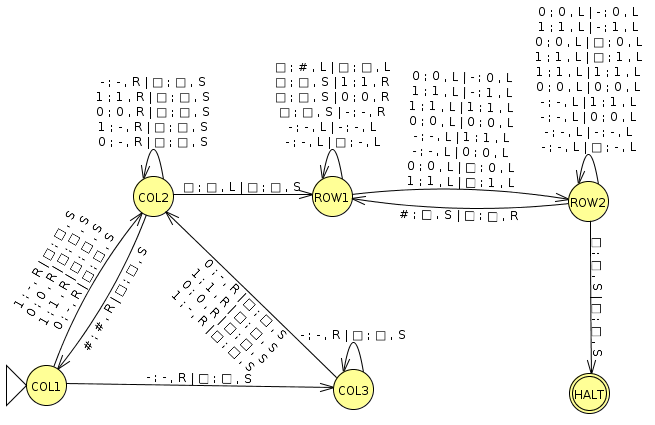
\includegraphics[width=0.9\textwidth]{bsp6_.png}
	  }
	  \caption{Turingmaschine}
	  \label{Labelname}
	\end{figure}
	
      \subsubsection{Pseudocode}
        Die NTM baut bei den Zuständen (COL1-3) auf das Prinzip von Guess and Check auf.
        Dabei wird der ganze Input nach der Reihe nach durchgegegangen. Die NTM schreibt zu Beginn eine 
        0 auf das zweite Band und haltet. Währenddessen wird das erste Band durchlaufen und alle Möglichkeiten ausprobiert, 
        indem man alle $2^{n-1}$ Möglichkeiten pro Reihe auf neuen TMs durchprobiert.
        
        Falls in einer Reihe nur '-' stehen, dann wird diese NTM verworfen, 
        da dies nicht nach
        den Regeln von Solitaire ist. Die NTM führt diesen Vorgang bis zum Ende der Eingabe fort. \\
        
        In der Zeile 2 des Pseudocodes finden wir eine big While-Schleife die 3 weitere innere Schleifen behinhaltet. \\
	$$\langle G \rangle =\overbrace{ \underbrace{Z_1}_{\substack{\longleftarrow \\ \longrightarrow  \\ \longleftarrow}} \# 
	\underbrace{Z_2}_{\substack{\longleftarrow \\ \longrightarrow  \\  \longleftarrow} }\# 
	\underbrace{Z_3}_{\substack{\longleftarrow \\ \longrightarrow  \\  \longleftarrow} }\# 
	\underbrace{Z_m}_{\substack{\mbox{1.1 inner while} \longleftarrow \\ \mbox{1.2 inner while} \longrightarrow 
	\\ \mbox{1.3 inner while} \longleftarrow} } }^{\mbox{1.big while} \longrightarrow} $$
        
        Wenn nun das Ende erreicht wird, arbeitet die NTM von hinten nach vorne Reihe nach Reihe ab. Sie kopiert die 
        letzte Reihe auf das zweite Band und vergleicht sie mit den anderen Reihen.
	\begin{table}[h]
	\centering
	  \begin{tabular}{|l||l|l|l|l|l|l|}
	  \hline
	  Rootband & 0 & 1 & 0 & 1 & 0 & 1 \\ \hline
	  Helpband & - & - & 1 & 0 & 0 & 1 \\ \hline 
	  \begin{tabular}[c]{@{}l@{}}Resulat auf \\ dem Helpband\end{tabular} & 0 & 1 & \multicolumn{2}{l|}{verwerfe} & 0 & 1 \\ \hline
	  \end{tabular}
	\end{table}
        
        Die NTM verwirft, sobald sie eine ungültige Konfiguration findet, oder haltet wenn sie alle Reihen verglichen hat.
        
        \newpage       
    
        \lstinputlisting[caption=Pseudocode zur NTM]{blatt6.py}
      
      
      \newpage
      \subsubsection{2. Ansalyse der Laufzeit}
      \setcounter{equation}{0}
      
	Für unsere Laufzeitanalyse berücksichtigen wir hauptsächlich die while-Schleifen, da diese die größte Bedeutung haben als
	Operationen wie Zuweisungen, Abfragen, etc \dots ( Man geht bei diesen Operationen davon aus, dass sie in konstanter
	Zeit ausgeführt werden können ). 
	
	\paragraph{\underline{Um die Analyse zu vereinfachen Teilen wir das Programm in 2 Teile:}}
	
	\subparagraph{1. Analysieren wir zunächst den ersten Teil des Pseudocodes:}
	
	Wir betrachten nun zunächst die erste while-Schleife ``1. big loop''. Diese Schleife iteriert über alle
	Zeilen des Spielfeldes und arbeitet somit in $\mathbb{O}(m)$ Zeit. (Zur Erinnerung: Das Spielbrett besitzt $m \times n$ Felder)\\
	
	Nun werden in dieser Schleife 3 weitere Schleifen, ``1.1 inner loop'', ``1.2 inner loop'' und ``1.3 inner loop'' ausgeführt. Betrachten
	wir zunächste die Erste der Drei:\\
	
	Wir erzeugen für Elemente in Reihe $Z_i$, in der wir uns gerade befinden $2^{n-1}$ Turingmaschinen, um eine nichtdeterministische Turingmaschine
	zu simulieren. (Man beachte, dass dies für die Laufzeitanalyse nicht bedeutsam ist, da nur die Simulation der NTM exponentielle Laufzeit besitzt!)\\
	
	In den 2 nachfolgenden Inneren Schleifen arbeitet die NTM alle erzeugten Turingmaschinen parallel ab. In diesen 2 Schleifen wird lediglich der Lesekopf
	zurückgeshiftet und dann die Regeln des SOLITAIRE, in der Reihe $Z_i$, überprüft. Da jede Zeile genau $n$ Elemente besitzt, ergibt sich somit für den
	ersten Teil der Analyse eine Laufzeit von
	\begin{equation}
	  T_1(n) = \mathbb{O}(m)*( \mathbb{O}(n) + \mathbb{O}(n) + \mathbb{O}(n)) = \mathbb{O}(mn) \\
	\end{equation}

	
	\subparagraph{2. Analyse des zweiten Teils:}
	
	Zunächst bemerken wir, dass die einzelne while-Schleife ``2. big loop'', nur vom Hauptband aufs Hilfsband kopiert, also $\mathbb{O}(nm)$ Zeit
	benötigt.(Gleiches gilt für das goto) \\
	
	Betrachten wir nun die for-Schleife, ``3. big loop'': \\
	
	Wir iterieren wieder über die Zeilen und dann über die Elemente in der Zeile also ergibt sich ingesamt $\mathbb{O}(mn)$ als Laufzeit hier. 
	( Die if Abfragen können wie oben bereits erwähnt in konstanter Zeit abgefragt werden )\\
	
	Insgesamt ergibt das für den zweiten Teil
	
	\begin{equation}
	  T_2(n) = \mathbb{O}(nm) + \mathbb{O}(nm) + \mathbb{O}(nm) = \mathbb{O}(nm).
	\end{equation}
	
	Die gesamte Laufzeit ist somit
	
	\begin{equation}
	  T(n) = T_1(n) + T_2(n) = \mathbb{O}(nm) + \mathbb{O}(nm) = \mathbb{O}(nm).
	\end{equation}
	
	 \textbf{Bemerkung.} Wenn wir OBdA annehmen $m\leq n$ ( ansonsten drehe das Spielbrett ) folgt $\mathbb{O}(nm) \leq \mathbb{O}(n^2)$ und somit ist die Laufzeit durch ein 
	Polynom 2ten Grades gegeben, daher eine polynomielle Laufzeit.\\
	
Damit haben wir also eine NTM, die in polynomieller Laufzeit SOLITAIRE entscheidet und somit folgt, dass die 
	Sprache SOLITAIRE in NP enthalten ist. \hfill $\square$
    \vfill
    
\end{homeworkProblem}


\end{document}